
\section{Application Evaluation}
\label{sec:apps}
Legion is a high-level runtime system that has been implemented on top
of our interface\cite{Legion12}.  
%The Legion runtime is distributed so 
%that there is an independent scheduler for each processor in the machine.  
The Legion programming model is built around the abstraction of 
{\em logical regions} which express locality and independence properties 
of data.  Computation in Legion is organized into a tree of tasks where 
each task must specify which logical regions will be accessed.
When executing a Legion task, the Legion runtime receives requests
to execute sub-tasks along with their region requirements.
This stream of tasks with region requirements is analogous to a stream
of instructions with register requirements that are executed by 
a hardware processor.  Hardware out-of-order processors are designed to
run ahead of the actual execution of a stream of instructions
to ensure that the processor's pipeline is fully utilized.  Similarly, in a
Legion application, for every processor there is an instance of the Legion runtime
that takes a stream of tasks with region requirements and asynchronously
runs ahead of the actual execution using a {\em software-out-of-order} (SOOP)
scheduler.  The SOOP leverages our interface by asynchronously issuing task launches, copy
operations, and synchronization operations that are chained together by
event dependences.  The full details of the SOOP are beyond the scope of this paper
and are described in \cite{Legion12}.

The fully asynchronous design of the interface that we've proposed in
this paper is crucial to Legion's SOOP implementation.  Without a fully
asynchronous interface, the SOOP would have to periodically invoke
blocking operations that would cause processors to stall and severly
limit Legion's ability to run ahead and keep the machine fully
occupied.  With a fully asynchronous interface the SOOP can run
far ahead of the actual execution, limited only by the physical resources
available in the machine, exactly like a hardware out-of-order processor.

In this section we demonstrate the performance properties of three
real-world applications that use the Legion runtime and the heterogeneous
implementation of our interface to run on the Keeneland supercomputer.
The three applications that we characterize are all multi-phase
applications that require parallel computation, data exchange, and
synchronization between phases. 
\begin{itemize} \itemsep1pt \parskip0pt \parsep0pt
\item {\em Circuit} is simulation of an irregular graph of integrated
circuit components connected by wires.  The graph is paritioned
and distributed across the machine.  Each time step performs is composed
of three phases that calculate currents on the wires, distribute charge between
nodes, and update the voltages of all ndoes.
\item Fluid - Is an incompressible fluid flow simulation from the PARSEC
benchmark suite\cite{bienia11benchmarking}.  When written in Legion, Fluid can
be run on distributed machines in addition to shared memory.  The Fluid simulation
models particles that flow through cells.  Each time requires multiple phases
that update different proprerties of the particles contingent upon neighboring
particles.
\item AMR - AMR is an adaptive mesh refinement benchmark based on the third heat
equation example from the Berkeley Labs BoxLib project\cite{BoxLib}.  AMR
simulates the two dimensional heat diffusion equation using three different levels
of refinement.  Each level is partitioned and distributed.  Time steps require
both intra- and inter-level communication and synchronization.
\end{itemize}
In Section~\ref{subsec:eventlife} we study the lifetime of events in
the Fluid application.  Section~\ref{subsec:lockmig} examines
the migration of locks in the Circuit application.  We give
a brief case study of reductions for the Circuit application
in Section~\ref{subsec:reduccase}.  Finally, we demonstrate
that the asynchronous nature of our interface is essential to the
performance of Legion by comparing to bulk-synchronous
implementations of our target applications in Section~\ref{subsec:bulkcomp}.
  
\subsection{Event Lifetimes}
\label{subsec:eventlife}
We instrumented the heterogenous implementation of our interface to 
capture information about events.  Figure~\ref{fig:eventlife} shows
the lifetimes of different types of events from a single run of the Fluid
application.  Dynamic events is a monotonically increasing line that
corresponds to the total number of events created in the system.  By
the end of the run, the simulation created over 260,000 dynamic
events.  In contrast, the physical events line corresponds to the total number
of generational events required to represent the dynamic events 
across all the nodes in the system.  Less than 5,000
generational events were required to represent all the dynamic events
illustrating that the technique of mapping from dynamic events to generational 
events described in Section~\ref{subsec:eventimpl} was effective.

The live event line shows the total number of {\em live events} at a point in time.  Dynamic events
are considered {\em live events} until their last query has been performed.  The number of live
events is equivalent to the number of physical events that would be required
in a reference counted scheme.  In this case we see that by reusing
generational events, we require up to 4X fewer generational events than would be
required by a reference counted scheme.

In an ideal world the total number of generational events required would be
equivalent to the maximum number of generational events in the untriggered
state at any point.  The untriggered event line shows the number of generational
events in the untriggered state.  We see that the total number of generational
events is actually slightly higher than the maximum number of generational
events in the untriggered state at any point.  The reason for this is that unused
generational events cannot be shared across nodes, so in some cases nodes must
make new generational events eventhough there are unused generational events
on other nodes.  The small difference in these lines shows that in practice
this is only a minor inefficiency.

\begin{figure}
\begin{center}
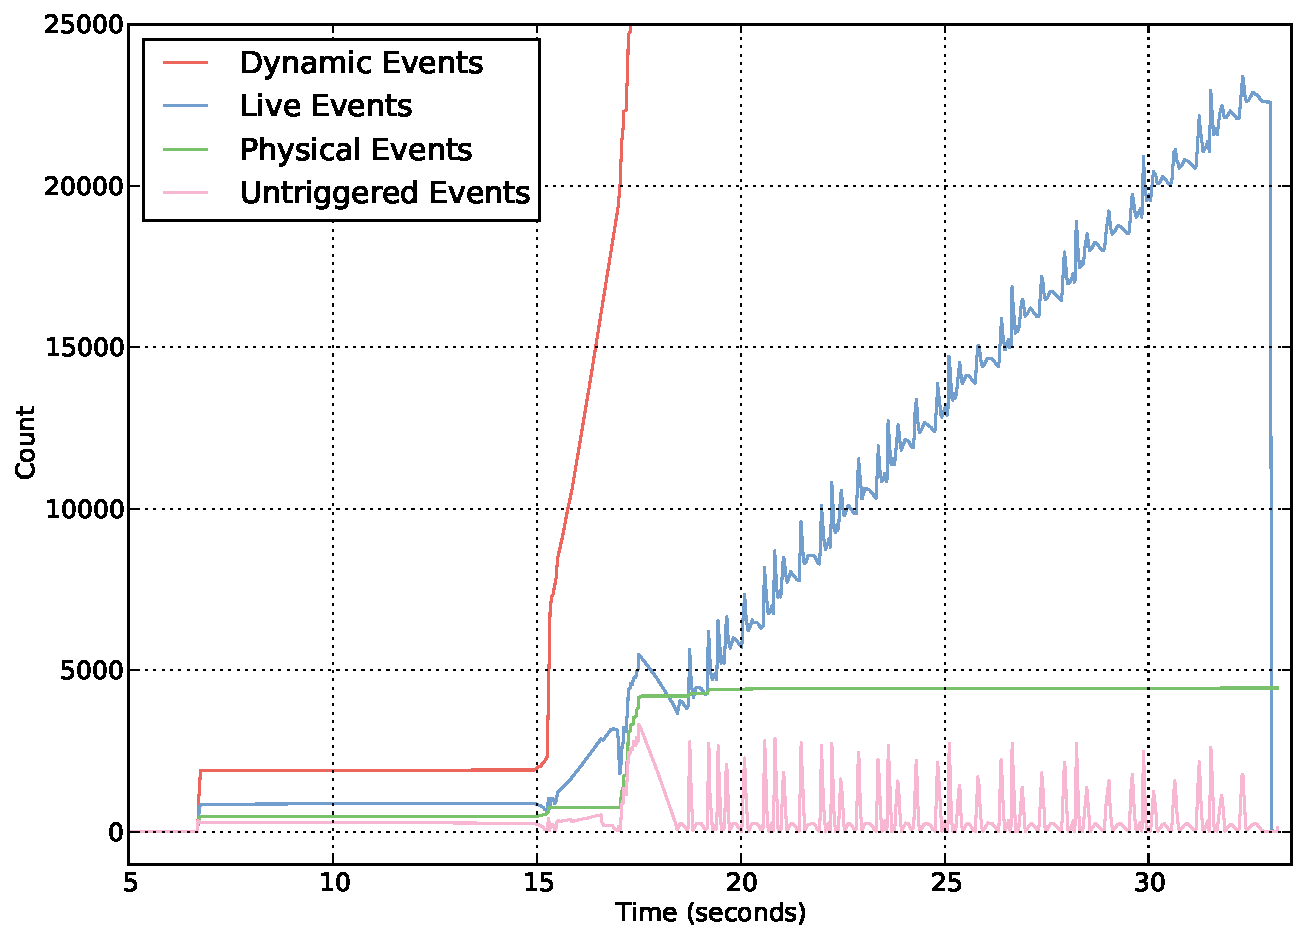
\includegraphics[scale=0.33]{figs/event_lifetimes.pdf}
\end{center}
\vspace{-6mm}
\caption{Event Liftimes - Fluid Application.\label{fig:eventlife}}
\vspace{-4mm}
\end{figure}

Figure~\ref{fig:eventlife} shows the event lifetimes in a run of the fluid application.  The total number
of events created during the application is over 260,000.

\subsection{Lock Migration}
\label{subsec:lockmig}
\begin{figure}
{
\renewcommand{\arraystretch}{1.2}
\begin{center}
\small
\begin{tabular}{c|rrrrrrr}
\multicolumn{1}{l}{\multirow{2}{*}{{\renewcommand{\arraystretch}{1}\begin{tabular}{@{}l}\bf Lock\\\bf Xfers\end{tabular}}}}
& \multicolumn{7}{c}{\bf Total Lock Requests} \\
     & 
\multicolumn{1}{c}{\bf 0} &
\multicolumn{1}{c}{\bf 1} &
\multicolumn{1}{c}{\bf 2-8} &
\multicolumn{1}{c}{\bf 9-16} &
\multicolumn{1}{c}{\bf 17-32} &
\multicolumn{1}{c}{\bf 33-64} &
\multicolumn{1}{c}{\bf 65-128} \\
{\bf 0    } & 45 & 2611 & 9   & 26   & 79    & 78    & 30     \\
{\bf 1    } &  -  & 450  &  -   &   -   &   -    &    -   &  -      \\
{\bf 2-8  } &  - & - & - & - & - & - & -\\
{\bf 9-16 } &  -  &  -    &   -  & 8 & - & - & -\\
\end{tabular}
\end{center}
}
\vspace{-6mm}
\caption{Locks by Request and Transfer Counts - Circuit Application.\label{fig:lockcount}}
\vspace{-4mm}
\end{figure}

\subsection{Reduction Case Study}
\label{subsec:reduccase}

\subsection{Bulk-Synchronous Comparison}
\label{subsec:bulkcomp}

